\documentclass[11pt]{article}

\usepackage[utf8]{inputenc}
\usepackage[T1]{fontenc}
\usepackage{amsmath}
\usepackage{indentfirst}
\usepackage[letterpaper]{geometry}
\usepackage{hyperref}
\usepackage{graphicx}
\usepackage{wrapfig}
\usepackage[bottom]{footmisc}
\usepackage{siunitx}
\usepackage{circuitikz}
\usepackage{array}
\usepackage{tikz}

\pagestyle{headings}

\begin{document}


\author{FJ Labs\footnotemark}
\title{FJ60BLX Component Choice and Analysis}
\date{August 21, 2020}
\maketitle

\tableofcontents

\newpage

\footnotetext{I would like to give special thanks to Hadi Iskandarani, his associated Discord group and Youtube channel, without whom this PCB design would have more errors than accuracies. As well, I would like to thank those kind enough to provide advice and support during the design stages of the board, answering my numerous questions without fail.}

\section{Introduction}

This document is intended to be a live document with a full description of the rationale for the primary component choices, the impetus behind why design choices were made, and an analysis of the availability and producibility of the components.

Major sections are divided into the core subsystems of the board starting from the core keyboard functionality then progressing to the additional functions added.

\section{Keyboard Overview}

The vision for the FJ60BLX PCB was to create an "all-in-one" PCB for the universal 60\% keyboards, including the KBDFans Tofu and 5Degrees cases, as well as similar generic cases. The primary feature draw of the keyboard is the Bluetooth functionality and full QMK support. Additional \emph{quality of life} features include under-glow RGB support and per-key backlighting. 

As such, the overarching theme of the design process has been to support Bluetooth in \emph{any way possible}. Much of the rationale behind each of the subsections follows from this core idea, and the remainder of the document should be read with it in mind.

\section{Microcontroller}

\subsection{Microcontroller Choice}

The main microcontroller for this board is the AT90USB646-MU. First and foremost, I address why this microcontroller was chosen over a smaller, cheaper, and more simple, Atmega32u4. For those knowledgable in keyboard PCB's, you will know the Atmega chip to be the bread and butter of keyboards. Unfortunately, this chip was simply not suitable for the FJ60BLX.

Let's first look at why the Atmega32U4 is so popular. First of all, it is a cheap, widely-produced microcontroller, which can easily be purchased under \$2 when produced at scale. Furthermore, it has most of the features necessary for operation under QMK, including 32KB of onboard flash memory and total of 26 I/O [input-output, GPIO] lines available. As well, it is a rather low-power device, consuming around $\SI{15}{\milli\ampere}$ at load when run with the usual specifications. It operates on a wide voltage range, functional from 2.7V to 5.5V. All these features make the chip ideal for a low-complexity device like a mechanical keyboard, whose sole purpose is to provide input and output.

\subsection{Why not the Atmega32U4?}

With that out of the way, let's talk about why I am \emph{not} using the Atmega32U4 for this keyboard, even though it seems like the perfect candidate.

The FJ60BLX consists of a matrix with rows and columns \([5,14]\). To maintain a proper matrix, as well as avoid ghosting of the keys, this, at minimum required 19 microcontroller pins. I am aware that alternative matrix combinations could have been arranged to reduce the number of pins needed (\emph{i.e.}, \([8,9]\)). However, this would not correspond logically to the actual layout of the keyboard, causing headaches when actually laying out the matrix, and even doing the keymaps in software. Thus, we are left with requiring 19 pins for the matrix.

For most boards, the Atmega32U4 can easily handle the 19 matrix pins without an issue (and that's why most boards use it). However, the FJ60BLX requires multiple additional pins, specifically for the Bluetooth support, under-glow, and backlight support. 

The Bluetooth module requires a minimum of 5 total pins (\emph{See supra., Bluetooth}). Additionally, RGB under-glow using addressable RGB LED's requires 1 pin (\emph{See supra, Under-glow}). Per-Key LED lightning using a common-cathode setup requires 1 pin (\emph{See supra, Per-Key LED)}. With this, our total pin count was brought up to 26 pins, the total available for the Atmega32U4 in terms of GPIO. Additionally, there are a few pins which are reserved for other purposes in the Atmega32U4 (\emph{i.e.}, Pin E2 (HWB)).

\subsection{Why the AT90USB646?}

As described above, the Atmega32U4 was likely not a suitable chip for this keyboard given the number of additional pins needed. Therefore, the search was on for an alternative chip. 

One of the primary drivers for the chip choice was QMK support. QMK, while being a great piece of software, has limited chip support\footnotemark \footnotetext{ \emph{See} QMK list of compatible microcontrollers at  \url{https://docs.qmk.fm/\#/compatible\_microcontrollers} }  due to its open-source nature. QMK supports two main types of microprocessors architectures, ARM and AVR. Immediately, ARM chips were ruled out, as I am not knowledgable about ARM, and do not wish to set too far out of my software comfort-zone, for a hardware project. 

Among the supported QMK AVR chips are the Atmega32U4 family, AT90USB646 family, and the Atmega32u2 family. Other AVR chips are also supported, but they do not use the LUFA USB stack, so they forgo native USB-support. Having ruled out the Atmega32U4, the Atmega32U2 family was also excluded due to even more reduced feature sets. Thus, we are left with the AT90USB646 family of chips.

The AT90USB646 family is class of chips which include the AT90USB646/647 and the AT90USB1286/1287. We'll first rule out the AT90USB1286/1287 lines. These chips contain 128KB of available flash memory (hence the product name). As QMK fits comfortable in even 32KB of flash\footnotemark \footnotetext{The Atmega32U[x] series has 32KB of flash and support QMK. Additionally, according to QMK documentation, 16KB flash chips are supportable, if features are selectively disabled from the firmware}, 128KB of flash was simply too much. We are then left with the AT90USB646/647 class.

The AT90USB646 and AT90USB647 are delineated by their USB interface version. The 646-type chips present the USB interface as a \emph{device} whereas the 647-type chips present the USB interface as a \emph{USB OTG} standard. Without diving much into the complexities of USB negotiation, the correct choice for a keyboard would be \emph{device} mode—the 646-type chips. Therefore, the final chip model was nailed down to the AT90USB646.

Of course, let's sanity check the chip to make sure it can do what we need. First of all, this chip has a total of 48 I/O lines, a much higher number compared to the 26 of the Atmega. Therefore, this chip can easily handle all the features we will throw at it. Additionally, this chip supports all the extra hardware features the Atmega32U4 does without sacrificing much. Power consumption is marginally higher, but this will be addressed in a later section.\footnotemark \footnotetext{\emph{See supra. Power Management}.}

\subsection{Package Choice}

The AT90USB646 is offered in 2 versions—a QFP and QFN package. To most, these package names seem completely foreign, but actually matter quite heavily during designing. The chips in each package are identical, but each package takes up a different amount of room of the circuit board when placed down. Therefore, care must be chosen when choosing a proper package for a chip, given constraints on board side and available room.

QFP [Quad Flat Pack] packages are very common and present themselves with exposed leads for each of the pins of the IC. \emph{See Figure 1} QFN [Quad Flat No-Leads] packages are much smaller packages, which do not have leads, but instead, have the connection points on the underside of the chip itself. \emph{See Figure 2}. 

\begin{wrapfigure}{r}{0.5\linewidth}
	\centering
	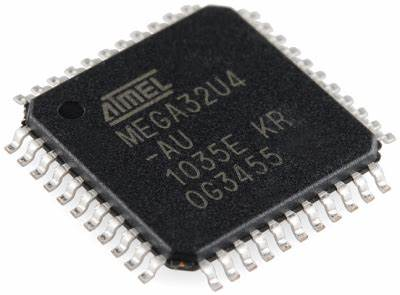
\includegraphics[width=3cm]{images/atmega32u4-qfp}
	\caption{Atmega32U4 in QFP.}
\end{wrapfigure}

\vspace{1.5cm}

\begin{wrapfigure}{r}{0.5\linewidth}
	\centering
	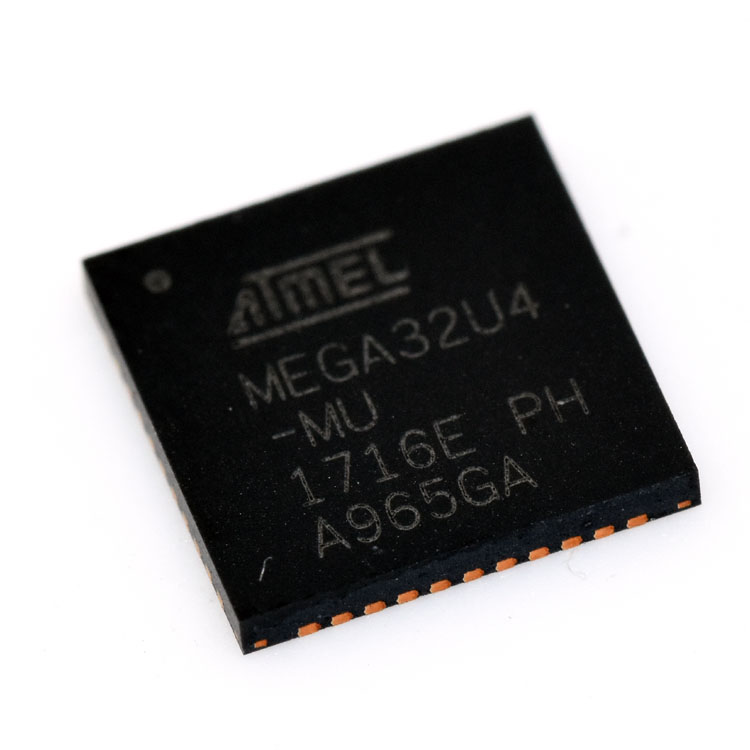
\includegraphics[width=3cm]{images/atmega32u4-qfn}
	\caption{Atmega32U4 in QFN.}
\end{wrapfigure}	

One of the primary constraints in package choice was that I wanted the microcontroller to sit squarely in between the Tab and Q keys. Partly, this was simply for a challenge. As well, I wished to avoid having to bring the USB data lines down below to somewhere with more space like around the spacebar. As the amount of space between those two keys is actually quite small, the natural choice was to go with the QFN package.

The QFN, given its size, is not without its drawbacks. Most notably, this chip is not hand-solderable in any sense of the imagination.\footnotemark \footnotetext{I am aware that drag-soldering is possible with a QFN package. However, without enough practice and also a very skilled hand, this is an incredibly difficult task. Even most professionals would regard this task as foolish.} Another drawback is the lack of ability to detect errors in manufacturing with this package type, as the solder pads are primarily below the chip itself. These problems will hopefully be remedied through functional testing by the PCB manufacturer themselves at additional cost.

\subsection{Component Availability}

This microcontroller is a widely used part and is not expected to face any component shortages. These can be purchased from most online component distributors as well as directly from the manufacturer. As such, no production challenges are expected from this chip choice.

\section{Bluetooth}

The Bluetooth chip of choice in this build is the Raytac MDBT40-256v3,\footnotemark \footnotetext{\url{https://www.raytac.com/product/ins.php?index\_id=63}} based off the Nordic nRF51822 ARM Cortex M0. To be brief, the reason this chip was chosen was off-the-shelf QMK support\footnotemark \footnotetext{I am not a C programmer, and I do not want to redevelop a Bluetooth implementation purely from scratch.} and reasonable cost. 

\subsection{Origins of this chip}

For those versed in QMK's documentation, you will know that QMK lists a few chips as \emph{supported} with the recommended being the Adafruit Bluefruit SPI Friend.\footnotemark \footnotetext{\url{www.adafruit.com/product/2633}}. Adafruit sells this module as a "breakout board" which is a pre-built carrier module for the chip as well as any supporting components. This sounds great! However, it is over \$15. Not great.

Instead, as the breakout board is simply a carrier board, I could easily rebuild the breakout board itself on the actual PCB, adding all the supporting components and main chip myself. \emph{I would like to give a huge shoutout to Adafruit for making not only their breakout boards available to the general public, but also their associated schematics.}\footnotemark \footnotetext{\url{https://cdn-learn.adafruit.com/assets/assets/000/026/205/original/adafruit\_products\_BluefruitLESPIFriend\_sch.png?1436186237}.}. Avoiding Adafruit's breakout board brings this chip down to around \$5 at scale per-chip and a few extra dollars for the surrounding supporting components. 


\subsection{Why this specific chip?}

The chip that Adafruit used for their breakout board is the MDBT40-256v3. Alternative versions of this chip are available as well, such as the MDBT40-P256v3 and MDBT40-256RV3. Differences between models are broken down in this section.

The difference between P and non-P models is the use of a chip antenna (non-P) vs a PCB antenna (P). Notably, chip antennas have greater signal strength and increased signal-to-noise ratio compared to their PCB antenna counterparts. In my original PCB vision, most boards would go into aluminum cases such as the Tofu, which tends to obstruct radio signals from passing through.\footnotemark \footnotetext{This effect is due primarily to the Faraday effect, with the case essentially acting as a Faraday cage, blocking RF in and out. A similar issue is faced with wireless charging and metal cases.} Therefore, signal strength was of \emph{utmost} importance when choosing the Bluetooth chip. Thus, P models were removed from consideration, despite being a tiny bit cheaper.

The difference between R and non-R models is the presence of extra RAM in the R models. Non-R models present a total of 16KB of useable RAM. This was determined to be sufficient as the Adafruit breakout board uses the non-R version and the Bluetooth chips will be running the identical Adafruit firmware. Therefore, R models were removed from consideration. 

The final model of this module being produced by Raytac is the MDBT40-256v3.

\subsection{Supporting Components}

The Bluetooth module chosen needs a few major supporting components to function properly in the FJ60BLX's circuit. These include a 5V-to-3.3V regulator and a level shifter. Most of the component choice was identical to that on the Adafruit breakout board, both due to simplicity as well as reliability and component availability. No future detail is given on the associated supporting components here.

\subsection{Component Availability}

The MDBT40-256v3 will be purchased through a direct purchasing relationship with the manufacturer. These chips are not readily available through component distributors due to rather niche nature. Instead, production supply has already been established and purchasing expectations have already been provided. Furthermore, purchasing directly from the manufacturer enables them to preprogram the chip with the requisite Adafruit firmware before assembly, saving time and error.

The supporting components are widely available from most component distributors. These are not in short supply and are quite generic in their nature. They may be swapped to equivalent components as many drop-in replacements exist. As such, they are not expected to be impediments to production.

\section{Power Management}

One of the most unique elements of the FJ60BLX is the inclusion of a multi-phasic power management scheme, built around Dynamic Power Path Management.\footnotemark \footnotetext{Dynamic Power Path Management (DPPM) is a T.I. specific branding of "Power Path Management."} As such, as a litany of additional components were added to support this, detailed in this section.

\subsection{Why DPPM?}

Most keyboards do not include a DPPM solution, so why did this keyboard need it? This was due to two competing electrical "dragons" in this board: 1) power savings due to being battery powered, and 2) high power draw due to the amount of LEDs. Most boards on the market are only faced with one of these dragons they need to contend with, instead of two completely mutually-exclusive ones.\footnotemark \footnotetext{Most boards with the amount of LED's present are only available in wired modes whereas most Bluetooth boards do not have so many LED's. Even notable boards like the Anne Pro 2 have fewer LED's than this board will have fully populated.} 

These two dragons have the following effects. A computer's standard USB port is typically limited to \(500mA\) of continuous current. Therefore, this acts as the upper ceiling of power draw from the board, to allow use when connected to USB and without a battery. The high amount of LED's will draw, at full load, a total of \(450mA\).\footnotemark \footnotetext{\emph{See supra, Under-glow} and \emph{Per-Key LEDs}} Therefore, to avoid LED's unfortunately being dimmed while simultaneously charging the battery, battery charging must be limited to \(50mA\) when LEDs are at full load. A typical 1800mAh battery, however will take:

$$ \frac{1800mAh}{50mA} = 36h $$

to achieve a full charge. This number is ridiculous and completely unacceptable for day-to-day use. Alternatively, power may have been divided equally between the battery charging and LEDs, leaving a \(250mA\) for both. This would give a battery charge time of:

$$ \frac{1800mAh}{250mA} = 7.2h $$

This is a much better result and somewhat more acceptable. What would be \emph{best} would be the ability to allow the LEDs to use as much power as they want, and redirect the entire remaining power budget of 500mA to the battery charger. Essentially, if a user turns off the LED's (\emph{e.g.,} before sleeping), the battery would be able to take advantage of almost all \(500mA\) power budget, giving a charge time of:

$$ \frac{1800mAh}{500mA} = 3.6h $$

This is a much greater result and is perfect for daily usage, with charging at night. This can only be accomplished with a Dynamic Power Path Management chip.

The primary ability of DPPM is to \emph{prioritize} system load from a total power budget, and redirect all remaining power for purposes of charging the battery. 

\subsection{Battery Charger}

Knowing that DPPM was required, the search for a battery charger chip was narrowed down.\footnotemark \footnotetext{The search for the chip was limited to Microchip chips as reliability was extremely important. Furthermore, Microchip provides immaculate documentation of their chips, providing detailed descriptions and implementation diagrams. I have also personally seen these chips in other products and Adafruit breakout boards, so I am aware of their basic implementation.} The Microchip MCP73871-2AAI/L was chosen as the final battery charger chip. 

This chip is a lithium-ion battery charger with integrated load-sharing power pathing (DPPM), with a total \(1.8A\) of input current, and \(1A\) charging. This was sufficient headroom over the maximum \(500mA\) power available through USB.\footnotemark \footnotetext{Alternative USB charging specifications are categorically not supported with this board. Any charger over 5V 500mA may have the potential to damage the board irreparably.} The feature set of this chip is extremely admirable, including all the needed features, plenty of headroom, and a large amount of programmable capability.

While such a powerful chip is, of course, not entirely necessary in the context of a DPPM charger circuit, their inclusion was certainly a plus. While many of the features were disabled or left unused, the system takes advantage of a handful. The charger offers built-in overheat protection, in the event that too much current gets drawn for the thermal capacity of the board. This will help prevent runaway charging fires common in poorly designed electronics. As well, the chip offers built-in automatic input-power switching, reducing overall component count and board space. Lastly, the amount of status LED's (while not on the final board design) will make circuit troubleshooting easy in the prototyping phases.

\subsubsection{Chip Models}

The MCP73871 is a family of chips that all offer the same basic functionality. Ultimately, the MCP73871-2AAI/L was chosen for its current availability (one of the only in the family that is available).

\subsubsection{Component Availability}

This chip appears to be widely available from most electronics components distributors as well as directly from the manufacturer. As such, no production challenges are expected from this chip choice.

\subsection{System Voltage and Power Conditions}

One of the biggest challenges with a battery powered system driving LEDs is power delivery. Lithium Ion batteries are known to produce a maximum voltage of \(4.2V\) and safe minimum voltage of \(3.0V\). In a very large amount of its battery life, the battery will operate at \(3.7V\). This is of slight concern as most RGB LEDs will operate at \(3.5V < V_f < 4.3V\). In other words, the LEDs may require up to \(4.3V\) to even turn on.

Clearly, running the entire system off a battery was not feasible. Therefore, voltage must be boosted to an acceptable level before being used by the system. 

It would be trivial to boost output voltage to \(5V\), but this presents drawbacks in terms of power efficiency. The AT90USB646 can draw as little as \(7.5mA\) at \(3.3V\) and a maximum of \(20mA\) at 5V. This presents a stark battery life contrast:

$$ \frac{1800mAh}{7.5mA} = 240h < \frac{1800mAh}{20mA} = 90h $$

This is a difference between running the keyboard for over a week and only 4 days. While the LED's can not run at 3.3V, a compromise can be made, at \(4.6V\). I chose not to skirt the minimum voltage of \(4.3V\) as diodes may present a forward voltage drop of typically \(200mV\): 

\begin{equation}
\begin{aligned}
V_{in} - V_{F} = V_{usable} \\
4.6V - 0.2V = 4.4V
\end{aligned}
\end{equation}

Additionally, as the Bluetooth module runs exclusively on 3.3V, the \(4.6V\) must be regulated down.\footnotemark \footnotetext{\emph{See infra. Bluetooth}} It's incredibly important to note that linear voltage regulators have a minimum voltage drop, defined as \(V_{Dropout} = V_{in} - V_{out}\). For the linear regulator chosen as part of the Bluetooth subsystem, the accompanying datasheet defined \(\max(V_{Dropout}) = 300mV\). Therefore, 

$$ \min(V_{In}) = V_{out} + \max(V_{Dropout}) = 3.3V + 0.3V = 3.6V $$

Clearly, this is in range of the \(V_{System} = 4.6V\) discussed earlier, so this subsystem is satisfied too. Furthermore, power loss (energy wasted as heat) on the system is fairly minimal given Bluetooth Low Energy's minimal power draw of around \(15mA\).

\begin{equation}
\begin{aligned}
P &= (V_{In} - V_{Out}) \times I \\
&= (4.6V - 3.3V) \times 0.015 \\
&= 0.0195W 
\end{aligned}
\end{equation}


Lately, of note is the interaction between battery power and USB power, in the presence of a DPPM. Previously mentioned, the DPPM chip will provide power to the system through the USB port when plugged in and via the battery otherwise. Thus, you are essentially left with two possible power conditions, \(3.0V \le V_{DPPM} \le 4.2V\) and \(V_{DPPM} = 5V \pm 0.25V\). 

So far, we have only looked at situations involving battery power. Reason being, the alternative power mode actually avoids most of the considerations previously mentioned. With \(V_{System} = 5V\), all LED's are easily driven. Furthermore, since the board is plugged in, battery life is not a concern. Lastly, the power loss of the Bluetooth chip is still quite minimal at \(0.0255W\). 

\subsection{Boost Converter}

Having decided on an appropriate system voltage, the final step was actually creating the voltage. It's important to note that battery voltage will always be lower than the system voltage, in other words, \(\forall V_{Batt}, V_{Batt} < V_{System}\). Therefore, in order to bring \(V_{Batt}\) to \(V_{System}\), we rely on a boost converter. The boost converter chosen was the TPS61252DSGT.

\subsubsection{Synchronous and Asynchronous Boost Converters}

There are two main types of boost converters available, synchronous and asynchronous. The basic method of operation of both is very similar, using energy stored in a magnetic field to provide additional voltage, with output voltage being controlled by a switching MOSFET that injects extra energy at the right time. The difference between the two boost "topologies" lies in the use of either a Schottky diode or a second MOSFET to control flyback current. 

As previously mentioned, all diodes have a forward voltage drop, \(V_F\). MOSFETs on the other hand behave similarly to "ideal diodes," theoretical one-way electric controls with a \(V_f \approx 0\). Asynchronous boost converters use a diode while a synchronous one uses a MOSFET. Recall how we also calculated power loss, which we can do similarly for an asynchronous converter, assuming an arbitrary \(V_{In}\) of a diode with a \(V_F = 300mV\), typical of Schottky diodes, and a current of \(500mA\).

\begin{equation}
\begin{aligned}
	P_{loss} &= (V_{In} - V_{Out}) \times I \\
	&= (V_{In} - (V_{In} - V_F) \times I \\
	&= V_F \times I \\
	&= 0.3V \times 0.5A \\
	P_{loss} &= 0.15W
\end{aligned}	
\end{equation}

While this may not seem like much, bear in mind that system at \(5V\) and \(500mA\) only consumes a power of \(2.5W\). This presents a 6\% power loss, a very inefficient design. A synchronous boost converter would have a power loss instead approaching zero, which is ideal. 

Therefore, in order to improve efficiency (and extend battery life), boost converter choices were limited to synchronous boost converters.

\subsubsection{Inductors and Switching Frequency}

As just mentioned, boost converters operate by storing energy in a magnetic field and later releasing this energy back into the circuit.\footnotemark \footnotetext{This arises out of Faraday's law of induction and Lenz's law.} The magnetic field is generated typically by an inductor. These are frequently seen as large windings of copper wire around a center core. While storing energy in the coil is great, if it is only stored and released once, that's not a useful change in voltage—that is merely a voltage spike, not at all helpful at driving components.

Instead, boost converters operate by storing and releasing energy from the magnetic field many hundreds of thousands of times a second. This gives boost converters the name "switch-mode power supply," effectively switching the coil on and off extremely frequently. If done fast enough, this produces close to a steady voltage at a higher level than input. 

The inductance (or amount of stored energy) is related closely to the switching frequency of the boost converter. If a switching frequency is lower, an inductor must store more energy (have a higher inductance) to bring the voltage back up to the target voltage. Conversely, a higher switching frequency requires a lower overall inductance. Higher inductance can be achieved through either a larger inductor or more coil windings.

As the board is fairly space constrained,\footnotemark \footnotetext{All power components were placed between the USB port and the Tab/Q keys. There was very little amount of room to work with.}, the inductor had to be quite small. Therefore, switching frequency had to be quite high to achieve the desired output voltage. Therefore, this limited boost converter choices to those operating above 1MHz.

\subsubsection{Part Choice}

Part consideration was narrowed down to Texas Instruments chips. This is due to previous experience using Texas Instruments boost converters for other projects. Additionally, since this component is extraordinarily critical to the rest of the board, reliability was vital and T.I. has a strong reputation in that regard. 

The final choice of the TPS61252 was due to its very high switching frequency of 3.25MHz, voltage adjustability, and high current rating. This chip also provides a unique mode known as "100\% Duty Cycle Mode." This mode activates if \(V_{in} > V_{System}\) (\emph{i.e.}, when connected to USB), allowing all power to bypass the boost converter entirely, achieving almost 100\% efficiency with near zero power loss. 

\subsubsection{Resulting Output Voltage}

The TPS61252 has a programmable output voltage, which operates on a feedback loop. According to the accompanying data sheet, the feedback loop is created through a resistor voltage divider, with the output voltage set by the following equation:

$$ V_{Out} = V_{FB} \times \left( 1 + \frac{R_1}{R_2} \right) $$

The data sheet further gives \(V_{FB} = 1.2V \) and we assume that \(R_2 = \SI{100}{\kilo\ohm}\)\footnotemark \footnotetext{This value is assumed as \(\SI{100}{\kilo\ohm}\) is used elsewhere on the board. \emph{See supra. Passives}.} Keeping our desired \(V_{Out} = 4.6V\) gives us:

\begin{equation}
\begin{aligned}
	4.6V &= 1.2V \times \left( 1 + \frac{R_1}{100000} \right) \\
	R_1 &= \SI{283.3}{\kilo\ohm}
\end{aligned}	
\end{equation}

Unfortunately, \SI{283.3}{\kilo\ohm} is not a readily available resistor value. Therefore, the closest resistor value was chosen, which came out to be \SI{270}{\kilo\ohm}. This gives a resulting \(V_{Out}\) of:

\begin{equation}
\begin{aligned}
	V_{Out} &= 1.2V \times \left( 1 + \frac{270000}{100000} \right) \\
	&= 4.44V
\end{aligned}	
\end{equation}

While this value is lower than our originally desired value of \(4.6V\), this is still within range for all functionality of the board and completely acceptable, using the calculations we ran through earlier in this section.

\subsubsection{Inductor Choice}

Inductor choice with this chip was very satisfying, requiring only a $\SI{1}{\micro\henry}$ inductor according to the data sheet. $\SI{1}{\micro\henry}$ inductors are extremely widely available in tiny package sizes, perfect for the space constrained board. 

However, inductance is not the only requirement to consider—amperage must also be taken into account. According to the accompanying data sheet, maximum current passing through the inductor may be calculated with the following set of equations:

\begin{equation}
\begin{aligned}
	I_L &= I_{Sys} + \frac{V_{In} \times D}{L \times f} \\
	D &= 1 - \frac{V_{in} \times \eta}{V_{Out}} \\
\end{aligned}
\end{equation}

$\eta$ is defined to be the estimated efficiency of the boost converter across all ranges, with the data sheet providing $\eta = 0.9$. Therefore, we can calculate $D$ as:

$$ D = 1 - \frac{3V * 0.9}{4.44V} = 0.3919 $$

We can then use this to get estimated inductor current required:

\begin{equation}
\begin{aligned}
	I_L &= 0.5A + \frac{3.0V \times 0.3919}{0.000001 \times 3250000} \\
	&= 0.862A
\end{aligned}	
\end{equation}

With this result, some additional buffer room was added, and the final inductor was selected to handle 1.5A. 

\subsection{Component Availability}

The TPS61252 appears to be widely available from most electronics components distributors as well as directly from the manufacturer. As such, no production challenges are expected from this chip choice.

\section{Under-glow LED's}

The FJ60BLX includes an under-glow LED subsystem (UG)\footnotemark \footnotetext{Under-glow is stylized with a hyphen in this document, as the alternative spelling fails spell-check. While no references for either stylization appears in reputable dictionary sources, the Supreme Court of Connecticut has preferred the non-hyphenated stylization in \emph{Borelli v. Renaldi}, No. AANCV146015474S, 2017 WL 5164609 (Conn. June 24, 2020). Why is this important? It is not.} using individually addressable RGB LED's. This section discusses why the specific LED's were chosen and some considerations for the subsystem as a whole. UG utilizes exclusively SK6805-E-J 1515 LED's.

\subsection{Design Constraints before Part Choice}

Before we can understand the part choice itself, we have to understand the design constraints were are working in. While the UG subsystem is still an independent subsystem, it necessarily interacts with all the microcontroller and power subsystems for its basic functionality. Below analyzes cross-subsystem interactions and the constraints they pose.

\subsubsection{Addressable vs. Unaddressable LED's}

\noindent{\textbf{A Brief Description of PWM}}

RGB LED's are able to produce an array of possible colors through a blending of three primary colors, red, blue, and green. To produce specific colors, the RGB LED will vary the intensity of its three individual color channels—for example; to get purple, you light red and blue at varying intensities and leave green off.\footnotemark \footnotetext{The above is a significant simplification of additive RGB color, useful only for its illustrative context in addressable and unaddressable LED's.}. You will frequently find such colors specified in RGB color notation, rgb(\(R,G,B\)) such that for \(\{x: R,G,B\}, 0 \le x \le 255\). In plain English, each red, green, and blue channel can range from 0 to 255 in intensity.

However, unlikely their antiquated cousins, the incandescent bulb, LED's are purely digital devices—they are either on or off. They are not able to "dim" to any arbitrary value as you might know if you ever used a normal light switch. However, this is not to say that \emph{apparent} brightness can not be changed. 

While avid PC gamers will scoff, the human eye has a limited "frame rate"\footnotemark \footnotetext{I am making a joke here, the human eye's "frame rate" is much higher than 240fps or whatever the cool kids use these days."} also known as the \emph{flicker fusion threshold}. At this threshold, the human eye will perceive a flickering source as a completely steady. While the exact threshold depends on each individual as well as variables relating to the light source itself, often this is around a few hundred Hz (flickers a second). 

LED's are able to take advantage of the flicker fusion threshold in order to change their \emph{apparent} brightness (\(b\)) while maintaining the same \emph{absolute} brightness (\(B\)). Assume an LED flickers with a frequency of \SI{1000}{\hertz} (\emph{i.e.} switches on-off 1000 times a second). The LED may spend a portion of its time Off (\(t_0\)) the the remainder of its time On (\(t_1 = 1 - t_0\)). An LED may achieve \(t_0 = t_1 = 0.5\) by turning on for 1/1000th of a second, followed by turning off for 1/1000th, and then on again. This would, due to the persistence of vision,\footnotemark \footnotetext{The fusion flicker threshold is a result of the persistence of vision.} the apparent brightness of the LED would be 50\%, \(b=0.5\). However, at any given moment, the absolute brightness of the LED would be at 100\% or 0\%, \(B=\{0,1\}\). 

This concept of varying the on time and off time of a digital element is known as Pulse Width Modulation (PWM), with a duty cycle of \(t_1\). Therefore, the above example would be at PWM with a duty cycle of 50\% or 0.5. We will denote this as \(f_{0.5}\). A PWM that is on for 75\% of the time would thus be denoted, \(f_{0.75}\).

\noindent{\textbf{RGB LED's and PWM}}

Now that we understand PWM, we can understand how an RGB LED modules its colors in the rgb() color codes. Simplifying a little, RGB codes can be first translated into percentages of each channel. For example, rgb(64,128,255) can be translated to rgb(25\%, 50\%, 100\%). This can then be translated into PWM notation as we now know that the Red channel needs to be at 25\% \emph{apparent} brightness, green at 50\%, and blue at 100\%. The resultant is rgb(\(f_{0.25},f_{0.5},f_{1}\)). This gives us a nice pastel blue. 

\

\noindent{\textbf{Unaddressable LED's}}

Unaddressable LED's are the most common type you find in LED strips and in general situations. They exist is two forms, common \emph{cathode} and common \emph{anode}. In common cathode LED's, the negative (ground) signal is shared among the RGB channels, and the positive channel is flickered at the required frequency. A common anode reverses, flicking each channels' ground at the required frequency. 

Therefore, to assign a color to a single unaddressable LED, you will need 3 microcontroller pins to PWM all three channels, regardless of the LED type. For 2 LED's, you will need 6 pins to be able to change colors independently. Obviously, this pin count adds up very quickly at a rate of \(3n\) the number of LED's. To get around this, most LED strips are therefore \emph{not} individually addressable. Instead, the PWM lines are shared among all LED's in the string, making the entire strip limited to one single color. This is clearly undesirable as you lose all those cool color effects.

\

\noindent{\textbf{Addressable LED's}}

Addressable LED's offer a unique solution to the problem we just presented with the unaddressable LED's. Instead of requiring a microcontroller to handle PWM for each of the channels, each LED will comes with an embedded controller handling the PWM aspects. The microcontroller is simply required to provide a binary data signal containing the color information in a format the controller understands. This simplifies our 3 line requirement down to only 1. These controllers offer additional pin saving, allowing LED's to be daisy-chained to each other in one long string. In a feat of creative engineering, this has allowed us to control a limitless number of LED's, each with different colors, using onto a single microcontroller pin. 

Clearly, addressable LED's were the clear choice for this keyboard (as well as most other keyboards out there). 

\subsubsection{Total Power Consumption}

The keyboard is limited to drawing a total of 500mA.\footnotemark \footnotetext{\emph{See infra, Power Management}.} Therefore, we must manage our total power draw carefully to avoid crossing this threshold. Typically, each single color LED will draw an \emph{absolute} maximum of 20mA with a typical current draw of 5mA. Most LED's are not set to draw 20mA as this amount of current is likely to damage the LED itself. The same is true for \emph{each} channel of an RGB LED, for a \emph{typical} max power consumption of 15mA.

We begin with a quick estimate of \emph{worse-case} power draw. We will assume there are a total of 65 Per-Key LED's\footnotemark \footnotetext{\emph{See supra. Per-Key LED's}} and there are 24 UG LED's. We can estimate total current as follows:

\begin{equation}
\begin{aligned}
	I_l &= I_t \times 65 + 3 I_t \times 24 \\
	&= 5 \times 65 + 15 \times 24 \\
	&= 685mA
\end{aligned}
\end{equation}

That is not good. Thankfully, we may use some clever tricks of human perception to reduce total power consumption. 

As discussed in length, RGB LED's are, in effect, 3 LED's in one, one for each channel. With all three channels at full brightness (\emph{i.e.,} rgb(\(f_{1},f_{1},f_{1}\))), this singular LED is essentially three times as bright as a single LED. This is entirely unnecessary and a completely waste of our power budget. Instead, what we can do it limit our \emph{total} combined channel duty cycle to 100\%.\footnotemark \footnotetext{Humans typically perceive different colors at different intensities, with green being the highest intensity color. Therefore, while this formula is illustrative, it is not necessary representative of the final software implementation for frequency brightness power modulation.} In effect, we can reduce this down to:

\begin{equation}
	f_R + f_B + f_G = f_1
\end{equation}

To maintain the correct color reproduction, the relative proportions of all three duty cycles must be kept the same. This is purely a software implementation and further details are out of scope for this document. Instead, we will modify our \emph{worse case} formula to assume the RGB LED's now only draw a maximum of 5mA, same as our per-key LED's. We then get:

\begin{equation}
\begin{aligned}
	I_l &= I_t \times (65 + 24) \\
	&= 5 \times 89 \\
	&= 445mA
\end{aligned}
\end{equation}

This result gives us plenty of headroom for the remainder of our subsystems such as the microcontroller, and bluetooth as well as inefficiencies throughout the circuit. If we assume that all other subsystems will consume 50mA combined, we see that 24 under-glow LED's is our maximum comfortable number. 

\subsection{LED Choice}

Know that we have these design constraints out of the way (24 addressable LED's), we can begin understanding part choice. 

The first primary choice note was QMK support. QMK provides support for WS2812 and data-signal equivalent LED's.\footnotemark \footnotetext{\url{https://docs.qmk.fm/\#/feature_rgblight}}. While there exist a litany of LED's that support this data signal, the ones that occupy nearly 100\% of the market share are the WS lines and SK lines. 

Initially, the WS2812 was the prime LED in consideration, being the most widely used addressable LED on the market. However, this was quickly dropped in favor of the WS2813, a sister product which had LED Bypass support. For most addressable LED's, the data signals for the LED's are daisy chained end to end. Therefore, if one LED were to fail or be damaged, the remainder of the string would fail as well. This could only be remedied by removing the LED and bridging the data in and out, effectively skipping the LED entirely. The WS2813, however, had a bypass feature, where it was not only chained to the next LED, but also the one over, allowing for a single LED failure in a string. 

Though initially extremely promising, form factor became a quick concern. My vision for the LED's on this board was to have a large number of them for the most even color possible. Frequently, under-glow LED boards have noticeable "hotspots" that are brighter than surrounding areas. Therefore, this board skirts the maximum amount of LED's allowable by power consumption, 24 LED's. This is higher than most, if not all, boards on the market. 

While most RGB LED's are in the 5050 form factor (5mm x 5mm), my expected LED density was simply too great to support that many large LED's. Therefore, I was limited to much smaller LED's. These did not exist in the WS lines, to my knowledge, so I began the search in the SK lines. I was immediately drawn to the SK6805-E-J, measuring only 1.5mm x 1.5mm. This was perfectly small enough to fit between individual key switches, while boasting the same maximum brightness as their larger counterparts. 

After checking compatibility (known supported according to QMK documentation), the SK6805-E-J was settled on as the final LED for underglow. 

\subsection{Component Availability}

The exact SK6805-E-J is, for some reason, notoriously difficult to track down. I found the exact component on Adafruit only, but this is clearly impracticable for larger productions. Instead, alternative equivalent parts were found, notably the TONYU 6805-5T. This part was individually qualified to meet the required specifications during my own testing and is the part incorporated into the final design.

This LED, as of time of writing, has 4,886 in stock at LCSC. This is enough for 200 boards, while more can be ordered in needed. Additional quantities are easy to acquire as this is a currently in-production component, and this is not expected to cause any production delays. 

\section{Per-Key LED's}

Per-Key LED's is a unique inclusion in this document, as it was a less of a component choice issue, but rather a design choice determination. While pre-soldered LED's will be offered as an option for this board, the exact component has not been narrowed down as of yet, and this document will \emph{not} reflect that component choice for flexibility. Much of the design regarding PWM and power consumption mimics that of the under-glow LED's and will not be discussed again for brevity.\footnotemark \\footnotetext{\emph{See infra. Under-glow LED's}}

\subsection{LED Form Factor}

A notable element of this board is the inclusion of both SMD and through hole LED support. SMD and through hole LED's have their own unique advantages. Notably, SMD LED's allows a PCB manufacturer to pre-solder the LED's to the PCB. I am aware that many in the keyboard community (me, included) do not enjoy the process of soldering 60 LED's, in addition to 60 switches. Therefore, the SMD LED option was geared towards those folks. A major disadvantage, however, of SMD LED's is that due to economies of scale, the PCB will only be offered in a single SMD LED color, with white being the most popular. Through hole LED's are much more customizable, letting each user choose the LED's they will be using, but on the other hand involve soldering. 

Therefore, to get the best of both worlds, both through hole and SMD pads were included on this PCB. On the base version of this board, the SMD pads will be unpopulated. A user is free to populate either the through hole LED's \emph{or} SMD pads, or not at all. Note that using \emph{both} through hole and SMD led's on one switch is not supported. However, they may be mixed and matched across multiple switches if desired.

\subsection{LED Specifications}

\subsubsection{Mechanical Specifications}

Ultimately, LED compatibility will depend entirely on your switches, especially SMD LED's. Note that most switches do not support SMD LED's. Compatible switches can be identified by a cutout on the bottom of the switch. All SMD LED's up to 0805 form factor are supported by the PCB itself, and generally up to 1.4mm height supported by switches.

For through hole LED's, 2.8mm, 3mm, and 5mm LED's are supported. While 5mm LED's may work, they may cause interference with keycaps and switches. Therefore, it is recommended to use 3mm through hole LED's if possible.

\subsubsection{Electrical Specifications}

As mentioned, this board operates at 4.44V nominally.\footnotemark \footnotetext{\emph{See infra. Power Management.}} Therefore, LED's with a maximum forward voltage under 4.4V are supported, which should encompass most common LED's on the market today. As typical with LED implementations, these LED's are wired in series with a current-limiting resistor. While we assumed that each LED will draw a maximum of 5mA in the previous section, we define this more rigorously below.

\subsubsection{Current Limiting Resistors}

We first begin this discussion noting that LED's are simply \emph{diodes} that happen to emit light (light-emitting diodes). We have discussed diode voltage drop calculations in a previous section,\footnotemark \footnotetext{\emph{See infra. Power Management.}} and will expand more with regards to current below.

Ohm's law provides us the guiding light when calculation our current limiting resistor. Ohm's law tells us that the current passing through a conductor between two points is directly proportional to the voltage between the two points. The constant of proportionality is the total resistance between the two points. This is summed into the famous formula:

$$ I = \frac{V}{R} $$

Next, we note that the complete circuit for a single LED presents a resistor and an LED in series, as per the figure below:

\begin{figure}[h!]
  \begin{center}
    \begin{circuitikz}
      \draw (0,0)
      to[V,v=$V_{sys}$] (0,2) % The voltage source
      to[short] (1,2)
      to[R=$R_1$] (3,2) % The resistor
      to[short] (4,2)
      to[full led] (4,0)
      to[short] (0,0);
    \end{circuitikz}
    \caption{Typical LED Series Current Limiting Resistor}
  \end{center}
\end{figure}

To calculate the total current flowing through the LED itself, our "two points" for Ohm's law calculation must start before the resistor and end after the LED. Ohm's law's "voltage" refers to the difference in voltage between the two points chosen, so we can therefore rewrite our Ohms law to reflect a diode's forward voltage drop:

$$ I = \frac{V_{sys} - V_f}{R} $$

We have already defined our system voltage, \(V_{sys}\) to be 4.44V volts and will be using 4.4V for future calculations. Next, we must determine the forward voltage drop for our LED's. This number, unfortunately, varies by both individual LED's and the color. A table of common \(V_f\) values is presented below.\footnotemark \footnotetext{Extracted from \url{https://stompville.co.uk/?p=37}}

\begin{center}
\begin{tabular}{ | c | c | }
	\hline
	\textbf{Color} & \textbf{Typical }\(V_f\) \\
	\hline
	Red & 1.7 \\
	Orange & 2 \\
	Yellow & 2.1 \\
	Green & 2.2 \\
	Blue & 3.2 \\
	White & 3.2 \\
	\hline
\end{tabular}
\end{center}

Given the spread of \(V_f\), we can not effectively regulate current, as each resistor is only capable of a single value resistance. Thus, we make some tradeoffs, in current regulation capacity in favor of manufacturability. We can calculate maximum and minimum resistor values to achieve a target current of 5V below:

\begin{equation}
\begin{aligned}
	I &= \frac{V_{sys} - V_f}{R_{max}} \\
	0.005 &= \frac{4.4 - 1.7}{R_{max}} \\
	R_{max} &= \SI{540}{\ohm} \\
	\\
	I &= \frac{V_{sys} - V_f}{R_{min}} \\
	0.005 &= \frac{4.4 - 3.2}{R_{min}} \\
	R_{min} &= \SI{240}{\ohm}
\end{aligned}
\end{equation}

Within this range, a value of \SI{300}{\ohm} was chosen. This value is notable as it allows use to 3 resistors in parallel to replace a \SI{100}{\ohm} resistor. As PCB manufacturing costs increase with the number of discrete passive components,\footnotemark \footnotetext{BOM consolidation is described in much greater depth in \emph{supra. Passives}.} using a nice round value was desirable. We can recalculate current drawn using a \SI{300}{\ohm} resistor for each of our above forward voltages, as well as calculate the maximum power draw for a total of 65 LED's. Detailed calculations are omitted for brevity, but they follow the previous Ohm's law formula exactly.

\begin{center}
\begin{tabular}{ | c | c | c | c |}
	\hline
	\textbf{Color} & \textbf{Typical }\(V_f\) & \textbf{Current } \(I_1\) & \textbf{Total Current}\\
	\hline
	Red & 1.7 & 9mA & 585mA \\
	Orange & 2 & 8mA & 520mA \\
	Yellow & 2.1 & 7.6mA & 494mA \\
	Green & 2.2 & 7.3mA & 474mA \\
	Blue & 3.2 & 4mA & 260mA \\
	White & 3.2 & 4mA & 260mA \\
	\hline
\end{tabular}
\end{center}

Those paying attention will notice that the total current draw for all but the Blue and White LED's exceed the maximum we allowed earlier of 5mA. This is a known issue with using a \SI{300}{\ohm} resistor, but we can get around this using PWM and some software. 

A factor not discussed earlier, the continuous current draw for a PWM circuit is proportional to the PWM duty cycle. We can represent this as:

$$ I_{c} = I_{t} \times f_{p} : 0 \le p \le 1 $$

with \(I_c\) representing continuous current draw and \(I_t\) representing the instantaneous total current by the circuit. USB power is able to supply an \(I_c\) of 500mA as mentioned through this document. However, \(I_t\) may be much higher due to the presence of multiple capacitors throughout the circuit as well as parasitic capacitance in the traces and passive components.\footnotemark \footnotetext{Detailed calculations of total energy storage in the power line capacitors and parasitic capacitance and inductance are omitted from this document in the interest of keeping it understandable and brief.} 


Given that PWM may be used both regulate brightness and continuous power draw, we can use software controlling the PWM signal to set a "maximum brightness," effectively \(f_{max}\). We can calculate \(f_{max}\) for each color, but this calculation is omitted for brevity.

To sum, the \SI{300}{\ohm} offers both flexibility in terms of LED's which can be used at maximum brightness, as well as serving a dual-purpose as a BOM consolidation item.

The astute among you may notice that these calculations were done with \(V_{sys} = 4.4V\) instead \(V_{sys} = 5V\) typical of USB power. I am aware of this discrepancy, with 5V increasing the maximum current draw of all the LED's. Again, this is easily remedied with PWM in software, and is not a critical design concern. The ease of use and reuse of a \SI{300}{\ohm} resistor in terms of manufacturability greatly outweigh the slight software burden in maintaining power consumption.

\subsection{Switching MOSFET}

Multiple mentions of PWM was made in this section. As discussed in the prior section, this involves a microcontroller switching a circuit on and off (more accurately, open and closed) thousands of times a second. However, most microcontrollers are simply not able to handle large amounts of current passing through them and will easily cook at the amount of current required for 65 keys. Therefore, we must take the PWM signal from a microcontroller and feed it into a high-power, high-frequency switch instead—a MOSFET. The following diagram shows a MOSFET being used to control a single LED, driven by a PWM signal at its gate. 

\begin{figure}[h!]
  \begin{center}
    \begin{circuitikz}
            \draw (1,0) to[short] (3,0);
            \draw (1.5,0.25) node[left]{Sig.};
            \draw (3,0.25) node[nigfete]{};
            \draw (-2,0) to[V,v=$V_{sys}$] (-2,2);
            \draw (-2,2) to[short] (-1.5,2);
            \draw (-1.5,2) to[R=$R_1$] (0,2) to[full led] (2,2)
            to[short] (3,2) to[short] (3,1); 
            \draw (3,-0.5) to[short] (3,-1.5) to[short] (-2,-1.5) to[short] (-2,0);
    \end{circuitikz}
    \caption{LED controlled by MOSFET}
  \end{center}
\end{figure}

Effectively, as the signal input on the gate is pulsed on or off, the MOSFET will either close the circuit (and the LED will turn on) or open the circuit (and the LED will turn off). Therefore, we are able to indirectly drive the LED, and do not have to risk any of the current flowing through our microcontroller itself which is providing the PWM signal. 

MOSFET's are commodity components and the generic FDN337N MOSFET was chosen for its ability to handle up to 1.3A while still remaining low cost and easily available.

\subsection{Component Availability}

Availability of passive components will be discussed in the later section.\footnotemark \footnotetext{\emph{See supra. Passives.}} The FDN337N MOSFET is a generic SOT-23 MOSFET and can be replaced with any equivalents in case of shortage. As only one MOSFET is needed to drive all LED's, component availability is not an issue with this component and is not expected to cause any production delays.

\section{Passives}

The following section will discuss a variety of passive components on the board, except for inductors\footnotemark \footnotetext{\emph{See infra, Boost Converter}}. While exact component choice is not discussed, since these passive components are extremely generic, design information is discussed.

\subsection{Resistors}

Two main form factors of resistors are being used on this board due to their differences in power ratings. All LED's use 0603 resistors capable of handling \(\frac{1}{8}\)W while all other resistors are using the 0402 form factor due to board space constraints. As neither of these packages are exceptionally hand-solderable, this PCB is relegated to pick-and-place assembly. 

Notably, 0603 resistors were chosen for LED's based on the minimum power loss the resistors must sustain without burning up. We can calculate the power loss of the resistors much like we did in the earlier sections\footnotemark \footnotetext{\emph{See infra, Power Management}} but we will describe the math behind the calculations more in depth here. 

We calculate power using a handy equation known as Joule's Law. This law tells us that Power in watts is proportional to the square of current and to resistance. This can be written as:

$$ P = I^2 R $$

Furthermore, we know from our previous discussions that Ohm's Law provides:

$$ I = \frac{V}{R} $$

or, rewritten:

$$ V = I R $$

With these two equations, we are able to rewrite Joule's Law to a more useable format for our purposes:

$$ P = I V $$

As we already know from our previous discussion on Ohm's Law, \(V\) is the difference in voltage between the two points of measurement, in our case, for LED's, \(V_{sys}\) and \(V_f\). Therefore, our final Joule's Law equation to calculate power loss across an LED current limiting resistor is given by:

$$ P = I (V_{sys} - V_f) $$

As our resistor needs only be specified to its maximum current rating, we can calculate the maximum power loss by inserting our worse case values. We assume that we will regulate \(I_c\) to be the actual value at \SI{300}{\ohm} \footnotemark \footnotetext{\emph{See infra. Per-Key LED's.}} simply to understand the absolute worst case scenario. Our worse case is given by:

\begin{equation}
\begin{aligned}
	P &= 0.009 \times (5 - 1.7)	\\
	&= 0.0297W
\end{aligned}	
\end{equation}

Note this power loss at the resistor is minimal and can easily be handled by a \(\frac{1}{16}\)W resistor. However, a \(\frac{1}{8}\)W resistor was chosen instead for added margin of error, allowing total max amperage to be 37mA at a 1.7V \(V_f\).

\subsection{Capacitors}

The role of a capacitor is to store charge for use at a later time, functioning similarly to an extremely small battery. In a simple keyboard PCB, the capacitors serve two main purposes, filtering and decoupling, and each function will be discussed briefly. All capacitors are in the 0603 form factor as it is the most flexible when it comes to amount of capacitance achievable in the form factor.

\subsubsection{Filtering Capacitors}

Capacitors are added to each of the main power lines to act as filters for any inbound power to the power management system. While power is frequently denoted in just a single voltage value, in the real world, imperfections in circuits, wires, and even the PCB itself may cause this value to fluctuate thousands if not hundreds of thousands of times a second. These dips can be a few mV to over a 100mV in certain situations. Therefore, proper filtering using capacitors is critical to stable power input and output.

In cases of a voltage sag, capacitors at power-line inputs will supply come of their stored charge to boost the voltage back to proper levels. In times when the voltage is at normal level, the capacitor will get recharged. Thus, we are left with a relatively stable voltage input line that is resistant to transient dips in voltages. The same is true for power-output lines coming out of the power management system. 

\subsubsection{Decoupling Capacitors}

Decoupling capacitors serve the same \emph{effective} purpose as their filtering counterparts, but in different circumstances. In many digital circuits, when certain switching tasks are performed, whether inside a microcontroller or by a MOSFET, sudden transient spikes in energy are required to flip the switch. This is somewhat analogous to the energy required to actually flick a stiff light switch. For the switching to happen at a rapid pace, these sudden spikes of energy must be provided quickly and should not bring down the voltage for the rest of the circuit (effectively causing voltage sag and ripple). 

To provide the sudden bursts of energy needed, decoupling capacitors are placed as close as possible to the components which require them, namely the microcontroller, Bluetooth chip, and each of the under-glow LED's.

Decoupling capacitors must be chosen and positioned very carefully. In the real world, a capacitor in a PCB has three main effects: capacitance, resistance, and inductance. In an ideal world, only capacitance would exist. However, we are forced to contend with the additional resistance (ESR) and inductance (ESL) created by both the internal construction of the capacitor and the PCB traces to the capacitor. Therefore, we want our capacitors as close as possible to the chip being decoupled to avoid the parasitic inductance and resistances found in PCB traces. 

\subsubsection{A Brief Dive into Component Theory}

The following is a highly technical dive into why the complexities of decoupling capacitors. Feel free to skip as this merely explains why multiple values of decoupling capacitors are necessary as well as keeping down trace lengths. 

As mentioned, real world capacitors have an effective ESR and ESL. Additionally, real capacitors have a total impedance, broken down into its ESR, its capacitive reactance, and inductive reactance. Both capacitive and inductive reactions are functions of frequency of the capacitor. The common formulas for each of these is given by:

\begin{equation}
	X_C = \frac{1}{2 \times \pi \times f \times c}	
\end{equation}

\begin{equation}
	X_L = 2 \times \pi \times f \times L
\end{equation}

\begin{equation}
	Z_{tot} = \text{ESR} + X_c + X_f	
\end{equation}

Our goal is to minimize the total impedance of the capacitor as impedance effectively slows down a capacitor's ability to respond to changes in voltage. Furthermore, all values in our function for total impedance are constants inherent to the capacitor itself, except for frequency of switching. Therefore, we can combine and simplify our equation for the total impedance as follows: 

\begin{equation}
\begin{aligned}
	Z &= \text{ESR} + \frac{1}{2 \times \pi \times f \times c} + (2 \times \pi \times f \times L) \\
	&= \alpha + \frac{1}{\beta f} + \gamma f \\
	\beta &= 2 \times \pi \times c \\
	\gamma &= 2 \times \pi \times L 
\end{aligned}
\end{equation}

We can then take the first-order condition of \(Z\) with respect to \(f\): 

\begin{equation}
	\frac{\delta Z}{\delta f} = \gamma - \frac{1}{\beta f^2} 
\end{equation}

With this first order condition,  we can see that total impedance falls initially with respect to frequency, due to the capacitive reactance effects. At the critical value where the capacitive and inductive reactances are equal, the total impedance is the lowest, given only by the ESR.\footnotemark \footnotetext{This point is the resonance frequency of the capacitor} Past this point, the total impedance will increase again due to the inductive reactance effects. Therefore, a real world capacitor really only a small window where its total impedance is rather low. \emph{See figure below.}\footnotemark

\begin{figure}[h!]
  \begin{center}
    \begin{tikzpicture}
        \draw [->, ultra thick] (0,0) -- (0,5) node[anchor=south east] {$Z_{tot}$};
        \draw [->, ultra thick] (0,0) -- (5,0) node[anchor=north west] {$f$}; 
        \draw (0,4) -- (2.5,1) -- (5,4);
        \draw [red, thick] (0,2) -- (5,2) node[anchor=west] {Acceptable Impedance};
    \end{tikzpicture}
    \caption{Total Impedance Graph for single capacitor}
  \end{center}
\end{figure}
\footnotetext{The industry standard representation of the impedance graph is linear, though in actuality, the graph is curved.}

This is behavior typically undesirable as the frequency of switching is difficult to predetermine. Instead, we want to extend the useful range of the capacitor itself. We are able to do this by placing multiple capacitors of different resonance frequencies in parallel, allowing whichever is able to respond the fastest to handle the load. Notably, capacitors with higher capacitance will have a lower resonance frequency and higher capacitance, a higher frequency. This is due to the reactive capacitance falling as capacitance rises. Therefore, using multiple capacitors, we are able to modify our response to the following figure. \emph{See Figure 6}.

\begin{figure}[h!]
  \begin{center}
    \begin{tikzpicture}
        \draw [->, ultra thick] (0,0) -- (0,5) node[anchor=south east] {$Z_{tot}$};
        \draw [->, ultra thick] (0,0) -- (9,0) node[anchor=north west] {$f$}; 
        \draw (0,4) -- (2.5,1) -- (3.5,1.5) -- (4.5,1) -- (5.5,1.5) -- (6.5,1) -- (9,4);
        \draw [red, thick] (0,2) -- (9,2) node[anchor=west] {Acceptable Impedance};
    \end{tikzpicture}
    \caption{Total Impedance Graph for multiple parallel capacitor}
  \end{center}
\end{figure}

As you can see, the usable frequency range for decoupling is significantly extended for each additional decoupling capacitor of a different value. While it may be tempting to add every possible capacitor value to cover all frequency ranges, the law of diminishing returns applies, as more capacitors will inevitably increase the trace length, adding additional inductance load to the total impedance.

Therefore, you'll commonly find decoupling and filtering capacitors in sets of three, a good number to balance the usable frequency range but low enough to be reasonable. 

\subsection{Diodes}

The diodes chosen for this board are the standard 1N4148WS diodes common to most, if not all, mechanical keyboards. The specification of these diodes is, frankly, unimportant as they will not be passing significant amounts of power. The switching speed is suitable for even the fastest of types (thousands of times a second) and are available in a wide variety of form factors. The diodes chosen are in the SOD323 form factor, instead of the flat leads,\footnotemark \footnotetext{This choice was purely due to personal preference and is of no functional important whatsoever.} and are extremely widely available.

\subsubsection{Component Availability} 

This diode is so widespread there may be diodes in stock than wanna-be celebrities in Los Angeles. No production delays are expected for this part. 

\section{Miscellaneous Components}

\subsection{USB Port}

The USB port chosen is the Korean Hroparts Elec Type-C-31-M-12. This is a 16-contact USB port, allowing for USB 3.0 operation. However, this keyboard only supports USB 2.0 speeds as it's merely a keyboard. This part was chosen primarily for its wide availability and high stock count. Additionally, the form factor is standard among mechanical keyboards and is frequently used in other designs.

\subsubsection{Component Availability}

This component is expected to be widely available currently and in the near future. No production delays are expected for this component, but alternative port options are available in the event this part is no longer available. No redesign is needed to accommodate alternative ports, and therefore, this component is not expected to cause any production delays.

\subsection{JST Connector}

This board uses a standard JST 2.0 PH right angle connector. This connector is typically found in the RC industry, widely used on single-cell lithium polymer batteries and small multi-cell ones. This connector was chosen for its standard sizing and ease of obtaining batteries. This is opposed to certain more niche sizes, which require additional adapters to fit common batteries. Furthermore, the right angle connector was chosen for clearance with the bottom of most cases, which is not large enough to hold straight connectors. 

Additionally, should a user wish to use a battery without the male connector, the onboard JST connector may be desoldered, allowing a user to solder the battery directly to the PCB. This \emph{is} a supported configuration.

\subsubsection{Component Availability}

This is a very common connector used in many industrial designs. Therefore, there is not expected to be any difficulty in sourcing this component. However, alternative compatible connectors have been identified. Therefore, this component is not expected to cause any production delays.

\subsection{Battery Protection}

This board includes an onboard battery protection chip, the FS312F-G. This chip provides protection for overcharging, overdischarging, and overcurrent. 

Lithium Ion batteries have a "safe" operating voltage—exceeding such limits may result in extreme safety hazards including fires, explosions, and toxic fumes. Therefore, preventing the excess of such safe limits is extremely critical in any battery operated circuit, a concept overlooked in other keyboard PCB's. The FS312F-G will stop current flow from an attached battery, should the battery voltage drop below 3V as well as will stop current if the battery voltage is over 4.3V. This is well within the safe window of all single-cell lithium ion batteries.

As this chip is specifically tuned to single-cell batteries, multi-cell batteries \emph{not} in a 2-battery symmetrical parallel configuration will irreparably damage this PCB. Using a 2-battery symmetrical parallel configuration is likely to be compatible, but \emph{this is an unsupported configuration and the user does so at their own risk.} The only supported configuration is a single, single-cell lithium ion or lithium polymer battery, with a nominal voltage of 3.7V and an instantaneous maximum voltage of 4.2V.

\subsubsection{Component Availability}

This chip (and surrounding componentss) is are generic and are widely used and available. Multiple alternative sources for this chip have been pre-identified and this chip is not expected to cause any production delays.





\end{document}
